% reset section counter
\setcounter{section}{0}

%\metadata{lecture ID}{Your names}{date}
\metadata{18}{Kaidi Cao, Ruocheng Wang}{Mar 17th, 2021}

% ===============================================

\sec{Review and overview}

In the last lecture, we completed our discussion of online learning and returned to the topic of algorithmic regularization. We described an instance of algorithmic regularization in the classification setting: gradient descent converges to the direction of the max-margin solution.

In this lecture...

\sec{Stochasticity in algorithmic regularization}
We note that in general, when the loss has multiple global minima, any decisions we make about the optimization algorithm will make a difference. Another important source of algorithmic regularization (possibly the most important) comes from the \textit{stochasticity} in the stochastic gradient descent (SGD) algorithm, where the parameters are optimized by updates of the form
\begin{equation}
\theta_{t+1} = \theta_t - \eta(\nabla\hat{L}(\theta_t) + \xi_t),
\end{equation}

where $\xi_t$ is a random noise term, typically with $\E\left[\xi_t\right]=0$ so the noise will not affect the result too much. The variance of $\xi_t$ can sometimes be time-dependent: for example, $\xi_t$ could be dependent on the parameter $\theta_t$. 

In practice, it turns out that larger gradient noise can lead to better generalization performance, as long as the algorithm can optimize under such level of noise. The intuition behind this phenomenon is that SGD converges to a ``flat'' global minimum, i.e. one with small curvature and small noise covariance. On the other hand, if you have a ``sharp'' local/global minimum with a large amount of noise, SGD will not converge to it stably. There are a number of works on this topic~\cite{haochen2020shape,blanc2020implicit}, but a lot of questions in this space remained to be answered.

\sec{Lipschitzness of models and generalization}
It has been found that the Lipschitzness of the model plays an important role in algorithmic regularization. As an illustration, note that the curvature (Hessian) of the loss function, the Lipschitzness of the model, and the noise level in SGD are all closely-related. To give a sense of the connections between them, suppose we have a model $f(x; \theta)$, a single example $(x, y)$, and a loss function $L(\theta) = \ell (f(x), y) = (f(x) - y)^2$. In this setup, we have the decomposition
\begin{align}
\nabla^2 L(\theta) = \underbrace{{\frac{\partial^2 \ell}{\partial f^2}}}_{\text{scalar}} \cdot \underbrace{\frac{\partial f}{\partial \theta}}_{\mathbb{R}^p} \cdot \underbrace{\frac{\partial f}{\partial \theta}^\top}_{\mathbb{R}^p} + \frac{\partial \ell}{\partial f} \cdot  \underbrace{\frac{\partial^2 f}{\partial \theta^2}}_{\mathbb{R}^{p\times p}}.
\end{align}

This decomposition is useful because it has been found empirically that the second term is relatively small. This implies that the Hessian is somewhat dominated by the first term. The first term, especially $\frac{\partial  f}{\partial \theta}$, relates to the Lipschitzness of the model with respect to the parameter. (There are similar connections between other quantities.)

Our algorithmic choices (e.g. SGD) seem to prefer Lipschitz models\footnote{By this we mean the Lipschitz constant of the model is small. Also, we are not distinguishing between the Lipschitz constant w.r.t to the input and that w.r.t. to the parameter because they are actually related (not covered in the lecture).}, which implies that such models generalize better. It remains to answer the question: \textbf{Why do Lipschitz models generalize better than arbitrary networks?} We want to theoretically analyze the relationship between Lipschitzness and generalization performance, and derive some generalization bounds w.r.t to the Lipschitzness of the models.

First, we note that the idea of using Lipschitzness to obtain generalization bounds is not new: it is the core of non-parametric statistics. However, such bounds suffer from the ``curse of dimensionality'', that is, the sample complexity grows exponentially as the data dimension $d$. Thus, using only Lipschitzness property is not enough to explain the generalization performance of neural networks: we need the help of parameterization. 

Consider a deep neural network $f(x) = \sigma(W_r\sigma(W_{r-1}\cdots \sigma(W_1x)))$ for binary classification. Recall, \cite{bartlett2017} showed that:
\begin{equation}
L(\theta) \leq \frac{R_S (\cF) }{\gamma},
\end{equation}
where $\gamma$ is the margin of the model, and $R_S (\cF)$ is some complexity that satisfies
\begin{equation}
R_S (\cF) \leq \underbrace{\l(\prod_{i=1}^r\|W_i\|_{\textup{op}} \r)}_{\text{relatively large}} \cdot \underbrace{\l( \sum_{i=1}^r\frac{\|W_i^T\|^{2/3}_{2,1}}{\|W_i\|_{\textup{op}}^{2/3}}\r)^{3/2}}_{\text{relatively small}}.
\end{equation}
The first term is essentially the upper bound on the Lipschitzness of the model w.r.t. to the input over the entire space. 

The limitation of this bound is that if $\norm{W_i}_{\textup{op}} >1$, then it grows exponentially in depth. On the other hand, if $\norm{W_i}_{\textup{op}} < 1$, then the $f_\theta(x)$ is exponentially small. Thus, it is very hard to make the spectral norm small while keeping the margin large. In the typical case, we have
\begin{align}
    \norm{W_1x} &\approx \norm{W_1}_{\textup{op}}\norm{x}, \\
    \norm{\sigma(W_1x)} &\approx \frac{1}{\sqrt{2}}\norm{W_1}_{\textup{op}}\norm{x}.
\end{align}
(The second approximation comes from the heuristic that the ReLU function $\sigma$ will zero out about half of the entries.) Thus, heuristically the output shrinks by a factor of $\sqrt{2}$ when passing through each layer. To make the output $f(x)\approx \Theta(1)$, we need $\norm{W_i}_{\textup{op}}\approx \sqrt{2}$, which makes the generalization bound very large. 

The deeper cause to this problem is that $\prod_i \norm{W_i}_{\textup{op}}$ is a worst-case bound on the Lipschitzness of models, since it is data-independent and assumes that the input spans over the entire space. Thus one way to improve the bound is by replacing ``worse-case Lipschitzness'' with the Lipschitzness at the data points $x^{(1)}, \cdots, x^{(n)}$. This also allows us to estimate the Lipschitzness on the empirical data, and gives us a regularizer roughly in accordance with what SGD prefers.

We want to prove a bound of the form
\begin{equation}\label{lec18:eqn:data_dependent}
L(w)\leq \text{poly}(\text{Lipschitzness of $f_w$ on $x^{(1)}, \cdots, x^{(n)}$}, \text{norms of $W_i$'s}).
\end{equation}
The RHS of \eqref{lec18:eqn:data_dependent} can be used as an explicit regularizer in model training to improve the generalization performance. 

\subsec{Proving data-dependent generalization bounds}
Before we prove a bound in the of form \eqref{lec18:eqn:data_dependent}, we first discuss why classical uniform convergence does not work. Note that the RHS of \eqref{lec18:eqn:data_dependent} is dependent on random variables $x^{(1)}, \cdots, x^{(n)}$. But typical bound of uniform convergence using Rademacher complexity is in the form
\begin{equation}
\forall f \in \cF,\quad L(f) \leq \text{comp}(\cF, n),
\end{equation}
where $\text{comp}$ is some complexity measure, or in the form
\begin{equation}
\forall f \in \cF, \quad L(f) \leq \text{comp}(f, n).
\end{equation}
The second bound can be achieved by defining $\cF_C= \{f: \text{comp}(f, n)\leq C\}$ first, applying the first type of bound for the class $\cF_C$, then performing a union bound over $C$. However, this approach does not work for obtaining a bound like the RHS of~\eqref{lec18:eqn:data_dependent} because the the corresponding hypothesis class is
\begin{equation}
\cF_C = \l\{f: \text{comp}(f, \{ (x\sp{i}, y\sp{i}) \}_{i=1}^n, n) \leq C \r\}.
\end{equation}
There are random variables in the definition of the hypothesis class, which is not allowed for Rademacher complexity. Hence, we cannot leverage such techniques directly.

To tackle this issue, we introduce a refined version of uniform convergence. Suppose we can decompose the complexity measure into the sum of a property related to each data point and the function we care about:
\begin{align}
\text{comp} \l(f, \{x^{(i)}, y^{(i)} \}_{i=1}^n, n \r) = \sum_{i=1}^n g((x^{(i)}, y^{(i)}), f).
\end{align}

We can define the \textit{augmented loss} as

\begin{align}
\Tilde{l} (f) = l(f) \cdot \bm{1} (g((x, y), f) \le C).
\end{align}

This means that we are changing the loss function to include the data-dependent term. An intuitive example can be found in Figure~\ref{lec18:fig:surrogate_loss}, where we have an empirical loss with very bizarre behavior, but only outside the low complexity region that we really care about. The augmented loss notices this and ``smooths out'' the irregularities outside the low complexity region by ignoring those terms.

\begin{figure}[htpb]
    \centering
    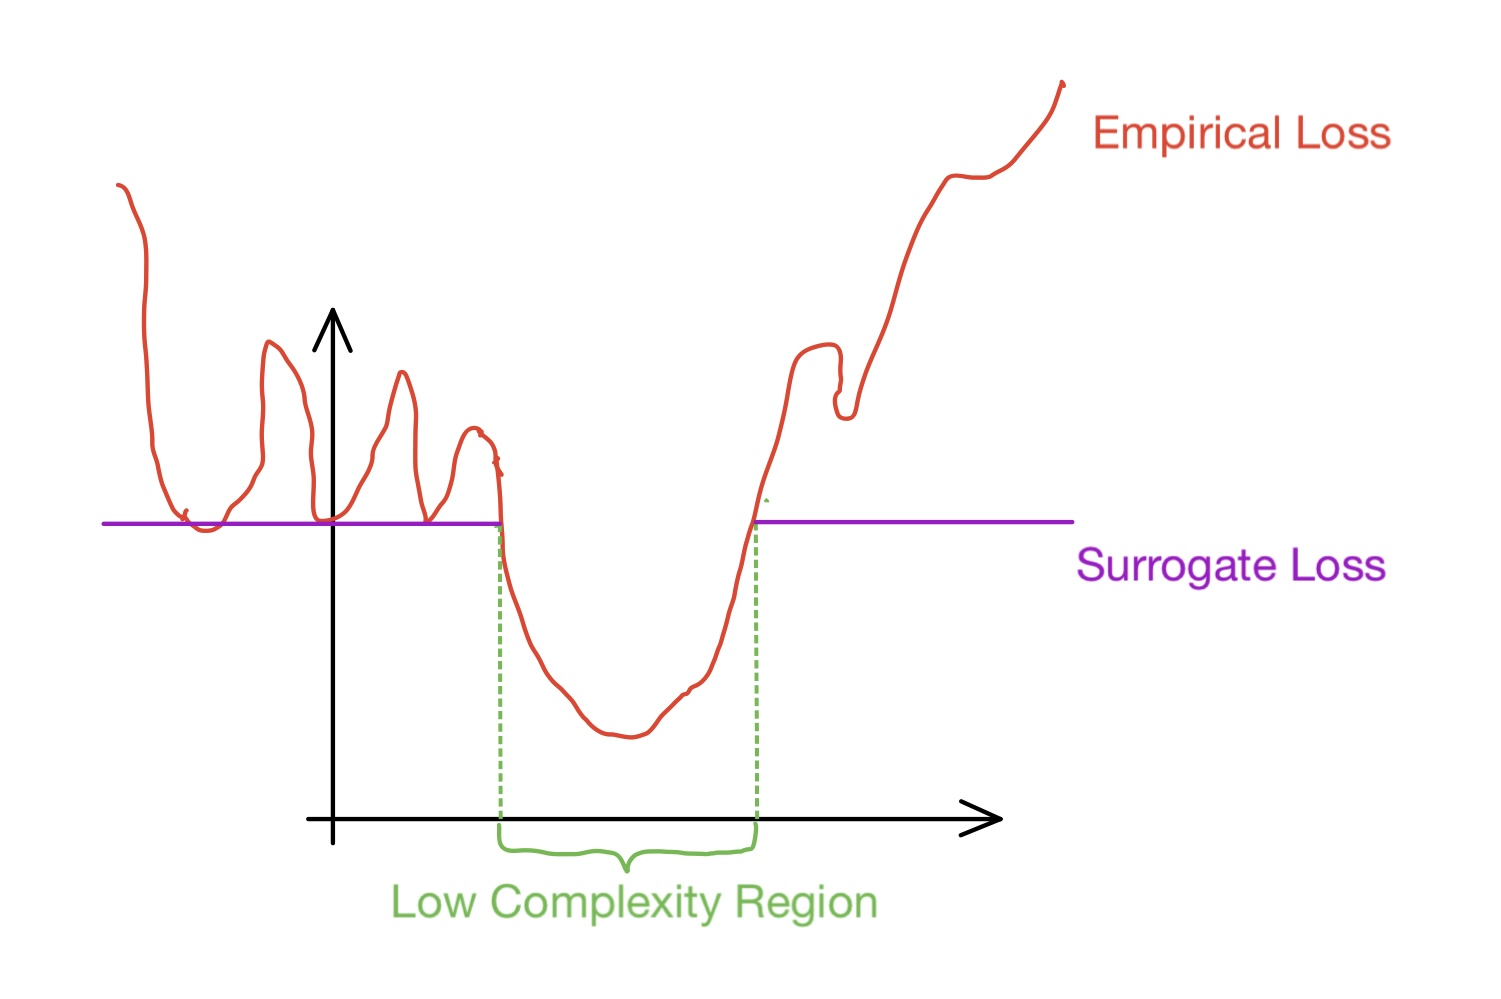
\includegraphics[width=0.7\textwidth]{figures/surrogate_loss.jpg}
    \caption{The empirical loss has bizarre behavior, but only outside the region of interest. The general idea is to define a surrogate loss and prove uniform convergence over the surrogate loss so as to avoid the bizarre behavior of the empirical loss.}
    \label{lec18:fig:surrogate_loss}
\end{figure}

The difficulty with taking this approach is that the low complexity region is random: if it was fixed, we could just zoom into that region and prove something directly by uniform convergence. We deal with this difficulty by defining a \textit{surrogate loss} which it could just be constant outside of the low complexity region. We may then apply uniform convergence over the entire space.

We have talked about the notion of surrogate losses before in this class. For example, the margin loss/ramp loss is a type of surrogate loss. There, we thought of using the surrogate loss to make the zero-one loss more continuous. Here, we use the surrogate loss to avoid dealing with the loss function in ``bad'' regions. Let us define a generalized version of margin loss:

\begin{definition}[Generalized margin]
Let $f : \R^d \mapsto \R$ be a classification model. We call $g_f(x, y)$ a \textit{generalized margin} if $g_f(x,y)$ satisfies
\begin{align}
    g_f(x, y) = \begin{cases} 0 &\text{if } f(x)\cdot y \le 0 \quad \text{(wrong prediction)}, \\  > 0 &\text{if } f(x)\cdot y > 0. \end{cases}
\end{align}
\end{definition}

Given this definition, we have the following lemma:
\begin{lemma}[Generalization bound for general margin]
\label{lec18:lem:generalizedmargin}
Suppose $g_f$ is a generalized margin. Let $G = \{ g_f : f \in \mathcal{F} \}$, and assume we have an $\epsilon$-covering of $G$ under the $\norm{\cdot}_\infty$ metric, $N_{\infty} (\epsilon, G)$, with $|N_{\infty} (\epsilon, G)|  \le \lfloor R^2 / \epsilon^2 \rfloor$, where $R$ is the Rademacher complexity of the model.

Then with probability larger than $1 - \delta$ over the draw of training data, $\forall f \in \mathcal{F}$ that correctly predicts the labels on the training data, we have
\begin{align}
    \Err (f) \le \tilO \l( \frac{R}{\min_i g_f(x^{(i)}, y^{(i)})} \cdot \frac{1}{\sqrt{n}} \r) + \tilO \l(\frac{1}{\sqrt{n}} \r).
\end{align}
\end{lemma}

The proof is similar to that for the bound we proved with margin loss earlier in the class, with only a few technical details changed.

\subsec{All-layer margin}

To use Lemma~\ref{lec18:lem:generalizedmargin}, we want to design a generalized margin $g_f(x, y)$ such that $G = \{ g_f : f \in \mathcal{F} \}$ has low complexity. We want this margin to capture the Lipschitzness of the model so that the bound will not scale badly in the worst case. If we use the standard margin $g_f(x, y) = yf(x)$, then $G$ depends on $\prod_i \| W_i \|_{\textup{op}}$; our goal is to do something better than this. To do so, we want to somehow have the margin depend on Lipschitzness.

The \textit{all-layer margin}~\cite{wei2019improved} is one such margin. Consider a perturbed model, where $\delta = (\delta_1, ..., \delta_r)$ is the perturbation and the original neural network model is perturbed in the following way:
\begin{align}
    h_1(x, \delta) &= \sigma(W_1 \cdot x) + \delta_1 \| x \|_2, \\
    h_2(x, \delta) &= \sigma(W_2 \cdot h_1(x, \delta)) + \delta_2 \|h_1(x, \delta) \|_2, \\
    &\vdots \nonumber \\
    f(x, \delta) = h_r(x, \delta) &= \sigma(W_r \cdot h_{r-1}(x, \delta)) + \delta_r \|h_{r-1}(x, \delta) \|_2.
\end{align}

We can then define the margin of the model as 

\begin{align}
    m_f(x,y) \overset{\Delta}{=} \min_{\delta} \sqrt{\sum_{i=1}^r \|\delta_i \|^2} \quad \text{s.t. } f(x, \delta) y \leq 0 \quad \text{(incorrect prediction)}.
\end{align}

(It can be proven that $m_f$ is indeed a generalized margin.) Under this definition, $m_f(x,y)$ is large if $f(x)$ is large (i.e. correct) and $f$ is robust to perturbation of example $x$. The good property is that under this definition, the margin already captures some Lipschitzness of the model. Applying Lemma~\ref{lec18:lem:generalizedmargin} with $m_f$ gives the the following theorem.

\begin{theorem}[Generalization bound for all-layer margin]
\label{lec18:thm:alllayermargin}
With probability larger than $1-\delta$ over the draw of training data, 
\begin{align}
    \Err (f) \le \tilO \l( \frac{\sum_{i=1}^r \|W_i \|_{1,1}}{\min_i m_f(x^{(i)}, y^{(i)})} \cdot \frac{1}{\sqrt{n}} \r) + \tilO \l( \frac{1}{\sqrt{n}} \r),
\end{align}
where $\| W \|_{1,1}$ is the sum of the absolute value of entries of $W$.
\end{theorem}

This theorem implies that a larger all-layer-margin implies better generalization. To get a larger all-layer-margin, we should make the network more robust to perturbation, i.e. more Lipschitz.

\begin{proof}
We present just the main proof ideas here. To use Lemma~\ref{lec18:lem:generalizedmargin}, it suffices to show that
\begin{equation}
N_\infty (\epsilon, G) \leq O \l( \frac{\sum_{i=1}^r \| W_i \|_{1,1} }{\epsilon^2} \r),
\end{equation}
where $G = \{ m_f : f \in \mathcal{F} \}$. Let $\cF_1, \dots, \cF_r$ be a sequence of hypothesis classes (corresponding to each layer in the network), and let $\cF = \{ f_r \circ f_{r-1} \circ \dots \circ f_1: f_i \in \cF_i \}$. \cite{wei2019improved} prove the following lemma:

\begin{lemma}[Decomposition lemma]
\label{lec18:lem:decomposition}
Let $m \circ \mathcal{F} = \{ m_f : f \in \mathcal{F}\}$ denote the family of all-layer margins of function compositions in $\mathcal{F}$. Then
\begin{align*}
    \log N_\infty \l( \sqrt{\sum_{i=1}^r \epsilon_i^2} , m\circ \mathcal{F} \r) \le \sum_i \log N_\infty (\epsilon_i, \mathcal{F}_i).
\end{align*}
\end{lemma}

This reduces the problem to bounding the covering number for each layer which is much easier, since each layer is basically a linear transformation plus a non-linearity.
\end{proof}

\sec{Summary of the course}

In the first part of the course, we talked about Rademacher complexity and concentration inequalities. They are classical but important tools in statistical machine learning: any time we have i.i.d. data, we will have to think about concentration bounds. We then spent some time discussing deep learning theory, covering non-convex optimization and algorithmic regularization. Within algorithmic regularization, we talked about the implicit biases of the optimizers, as well as the generalization bounds for deep learning models. We also spent time on online learning theory, a more classical approach for dealing with domain shift and potentially adversarial data.